\begin{frame}[label=metho]{Methodology}
	\textbf{Project Pipeline}
	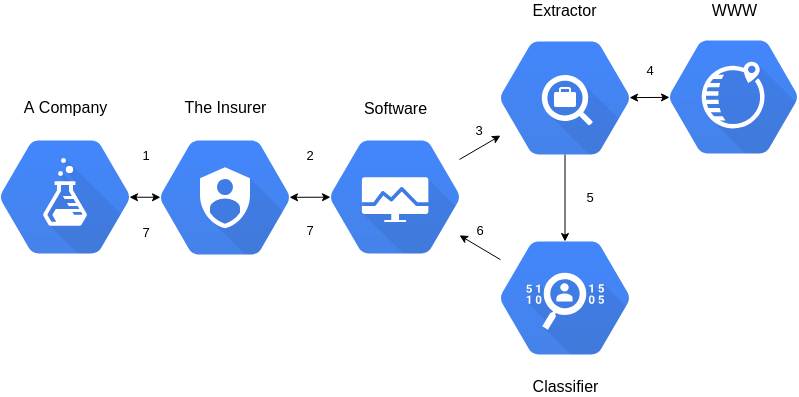
\includegraphics[width=\textwidth]{images/project_pipeline.png}
\end{frame}


\begin{frame}[label=metho]{Methodology}
	\textbf{The Extractor}
	\begin{itemize}
		\item Lot of work
		\item No Universal extractor
		\item Multistep extraction process
	\end{itemize}
\end{frame}


\begin{frame}[label=metho]{Methodology}
	\textbf{Extraction Example}
	
\end{frame}



\begin{frame}[label=metho]{Methodology}
	\textbf{Automating Extraction}
	\begin{itemize}
		\item Crawler and Scrapers
		\begin{itemize}
			\item Mimics the user by browsing without browser
			\item limitations: user interface design, dynamic rendered content and capcha
		\end{itemize}		
		\item Application Programming Interface (API)
		\begin{itemize}
			\item API based economy
			\item Communication contract
		\end{itemize}	
		\item Extraction Software should support both methods of extraction
	\end{itemize}	
	
\end{frame}



\begin{frame}[label=metho]{Methodology}
	\textbf{Using Textual Data}
	\begin{itemize}
		\item Linking key words to categories 
		\item Using the dynamic descendent classification framework
	\end{itemize}	
	
	\textbf{Dynamic descendent classifier}
	\begin{itemize}
		\item Machine Learning Algorithm trained to predict class based on words
		\item convert words into numeric vector
		\item generate a prediction based on the vector's values
	\end{itemize}	
	
\end{frame}


\begin{frame}[label=metho]{Methodology}
	\textbf{Training an algorithm}
	\begin{itemize}
		\item Classification is a task requiring supervised learning
		\item Requires a set of $N$ example with their good answer
		\item Calibrate itself to minimize loss function
	\end{itemize}	
	
	\textbf{Algorithm Trained by Supervised Learning}
	\begin{itemize}
		\item Be $\boldmath{X}$ a $N\times M$ matrix, with $N$ the number of example and $M$ features
		\item Be $\boldmath{Y}$ a $N\times1$ column vector, containing the associated values of the $N$ examples
		\item Let the algorithm \textit{learn} the $\beta$ that minimize the Mean Square Error in 
		$$ \boldmath{Y} = \beta\boldmath{X} $$
		\item Arguably, the $\boldmath{\beta}$ are obtained with the Maximum Likely Hood estimators
	\end{itemize}	
	
\end{frame}


\begin{frame}[label=metho]{Methodology}
	\textbf{Building a Training Data Set}
	\begin{itemize}
		\item Need to create a dataset 
		\begin{itemize}
			\item Linking a company occupancy code, as defined by a classification scheme
			\item To keywords extracted from a source
		\end{itemize}	
		\item The Dataset is source specific
		\item Small to Medium Data
	
	\end{itemize}	
\end{frame}


\begin{frame}[label=metho]{Methodology}
	\textbf{Not Using Big Data in Machine Learning}
	\begin{itemize}
		\item Unrelated, yet linked concept
		\item Machine Learning is the concept of training algoritmm for specific task
		\item Big Data refers to Data with usage problem due to the 4Vs
		\begin{itemize}
			\item However, value locked in big data can be accessed using Machine Learning
		\end{itemize}	
	\end{itemize}
\end{frame}


\begin{frame}[label=metho]{Methodology}
	\textbf{Data Set of Words}
	\begin{itemize}
		\item Not directly usable by machine learning algorithms
		\item NLP solves this problem
		\item Text Mining Software implements NLP findings
		\item Change a few blocs beneath the hood
		\item NLP Classification Pipeline
		\begin{itemize}
			\item Tokenization
			\item Transformation
			\item Classification
		\end{itemize}	
	\end{itemize}
\end{frame}


\begin{frame}[label=metho]{Methodology}
	\textbf{Tokenization}
	\begin{itemize}
		\item Split each document $d_i, i \in(1, N)$ into tokens $w_j, j \in (1, M) $ 
		\item In its most basic form, tokens generated $w_j$ are words
		\item Create a bag of words
		\begin{itemize}
			\item With the $J$ distinct tokens contained in the $N$ documents forming the corpus $D$
		\end{itemize}
		\item Creates an occurence matrix $S, N \times M$ with elements
		$$ s_{i,j} = 1 \textrm{ if } w_j \in d_i, 0 \textrm{ otherwise}$$
	\end{itemize}
\end{frame}



\begin{frame}[label=metho]{Methodology}
	\textbf{Occurence Matrix Example}
\end{frame}

\begin{frame}[label=metho]{Methodology}
	\textbf{Additional Tokenization Steps}
	\begin{itemize}
		\item Normalization
		\begin{itemize}
			\item Common writing for "same" word
			\item Restaurant vs Restaurants
		\end{itemize}
		
		\item StopWords
		\begin{itemize}
			\item Words that have no particular meaning
			\item I, if, then,...
		\end{itemize}
		
		\item N-Grams
		\begin{itemize}
			\item Combining consecutive n-tokens for additionnal meaning
			\item the tokens Machine and Learning vs the token Machine Learning
		\end{itemize}
		
		\item Part-Of-Speach Tagging
		\begin{itemize}
			\item Adding the syntaxic group to a words to remove ambiguity
			\item Live (verb) vs Live (adjective)
		\end{itemize}
		
	\end{itemize}
\end{frame}



\begin{frame}[label=metho]{Methodology}
	\textbf{Transformation Step}
	\begin{itemize}
		\item Adjust weigth for word relevance in the current task
		\item Classification task wants to maximise discrimination between $k$ classes.
		\item Add weigth to token that are usefull
		\item Remove weigth to token that are useless
		\item Metrics for usefulness
		\begin{itemize}
			\item Term-Frequence \ Inverse-Document-Frequency (TF/IDF)
			\item Bi-Normal Separation (BNS)
		\end{itemize}
	\end{itemize}
\end{frame}


\begin{frame}[label=metho]{Methodology}
	\textbf{Document-Frequencty / Inverse-Document-Frequency}
	\begin{itemize}
		\item Intuition
		\begin{itemize}
			\item Useless Word that do not carry meaning would appear in any document, regardless the category
			\item Usefull Domain related word should occur often in a document
		\end{itemize}
		\item formula here
	\end{itemize}
\end{frame}


\begin{frame}[label=metho]{Methodology}
	\textbf{Bi-Normal Separation}
	\begin{itemize}
		\item Intuition
		\begin{itemize}
			\item Words that occurs only in documents of a single category are usefull
			\item Words occuring randomly in documents are useless
		\end{itemize}
			\item formula here
	\end{itemize}
\end{frame}


\begin{frame}[label=metho]{Methodology}

	\textbf{True Positive Rate (TPR), False Positive Rate (FPR)}
	\begin{itemize}
		\item Example: $k=2$ classes, $N$ documents of known but hidden category
	\end{itemize}

			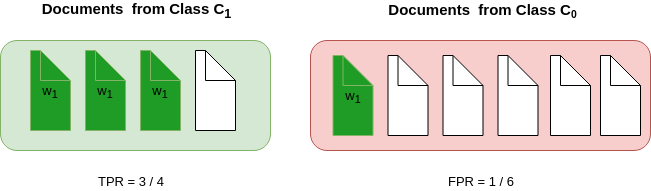
\includegraphics[width=\textwidth]{images/TPRFPR_example.png}

	\begin{itemize}
		\item Guess class $C_1$ for document $d_i, i = 1,...,N$ if $w_1$ is present.
			\item Amongs $n$ guessed docuement:
		\begin{itemize}

			\item \textbf{TPR} = number of documents $d$ that really belong to $C_1$ / the real number of documents belonging to $C_1$
			\item \textbf{FPR} = number of documents $d$ that do not belong to $C_1$ / the real number of documents not belonging to $C_1$
		\end{itemize}
	\end{itemize}

			


\end{frame}

\begin{frame}[label=metho]{Methodology}
		\begin{itemize}
		\item Given TPR = $\frac{3}{4}$ and FPR = $\frac{1}{6}$
			\begin{itemize}
				\item Very usefull word
				\item $\textrm{abs}(\Phi^{-1}(\frac{3}{4}) - \Phi^{-1}(\frac{1}{6}) ) > 1$ 
				\item Absolute value usefull for enhancing word that are uncorrelated
				\item $C_1$ and $C_2$ are somewhat arbitraty
			\end{itemize}
		\item Given TPR = 0.50 and FPR = 0.50
		\begin{itemize}
			\item Very useless word
			\item $\textrm{abs}(\Phi^{-1}(0.50) - \Phi^{-1}(0.50) ) = 0$ 
		\end{itemize}
	
	\end{itemize}
\end{frame}

\begin{frame}[label=metho]{Methodology}
	\textbf{Bi-Normal Separation}
	\begin{itemize}
		\item Limited to 2 classes (binary classification)
		\item Generalized to $n>2$ classes in this project
	\end{itemize}
\end{frame}


\begin{frame}[label=metho]{Methodology}
	\textbf{Classification Step}
	\begin{itemize}
		\item The actual machine learning algorithm
		\item Prior steps are mendatory preprocessing
		\item Data in matricial form $\boldmath{X}, \boldmath{Y}$ 
		\item Algorithms for classification
		\begin{itemize}
			\item Naive Bayes Classifier, Logistic Regression
			\item Support Vector Machine (SVM), Neural Network (DL)
		\end{itemize}
	\end{itemize}
\end{frame}


\begin{frame}[label=metho]{Methodology}
	\textbf{Naive Bayes Classifier}
	\begin{itemize}
		\item Very useful baseline algorithm
		\item Strong Hypothesis, but okay in NLP
		\item Given the class of the document, all features are independant
		\item Prediction formula
		$$\hat{y} = \arg\max P(C_k) \prod_{n}^{i=1}p(x_i|C_k)$$
		\item Where \textit{a posteriori} probabilities have been learned using the moment estimators
		
	\end{itemize}
	
	
	
\end{frame}




\begin{frame}[label=metho]{Methodology}
	\textbf{Logistic Classifier}
	\begin{itemize}
		\item A Stronger prediction algorithm, liberalized it's formula
		\item Prediction formula
$$ \hat{y} = \arg\max \beta_{K0} + \boldsymbol{\beta_{K}^T} \cdot  \boldsymbol{x} , $$
		\item Where the parameters have been learned by maximizing the likelihood score

	$$  l(\beta) = \sum_{N}^{i=1} y_i \beta^T x_i - \log(1+ e^{B^T x_i}) $$
		
	\end{itemize}
\end{frame}

\begin{frame}[label=metho]{Methodology}
	\textbf{SVM and DL}
	\begin{itemize}
		\item Surprise, no usage in this project
		\item More a proof of concept than an optimal implementation
		\item More black box and less room for digging in the depth of the data
		\item Questionable appropriateness
	\end{itemize}
\end{frame}


\begin{frame}[label=metho]{Methodology}
	\textbf{Choosing Between Many Categories}
	\begin{itemize}
		\item The classification Scheme has $K \geq 200$ classes.
	\end{itemize}

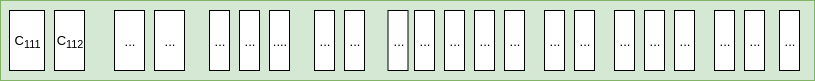
\includegraphics[width=\textwidth]{images/bottom_level.png}
	
	\begin{itemize}
	\item Example of classification
\begin{itemize}
	\item Restaurant - No Alcohol - Fastfood
	\item Restaurant - Alcohol - Steakhouse
	\item Service - Finance - Accounting
\end{itemize}
\end{itemize}



\end{frame}


\begin{frame}[label=metho]{Methodology}
	\textbf{Choosing Between Many Categories}
	\begin{itemize}
		\item Multiple level classification scheme 
	\end{itemize}
	
	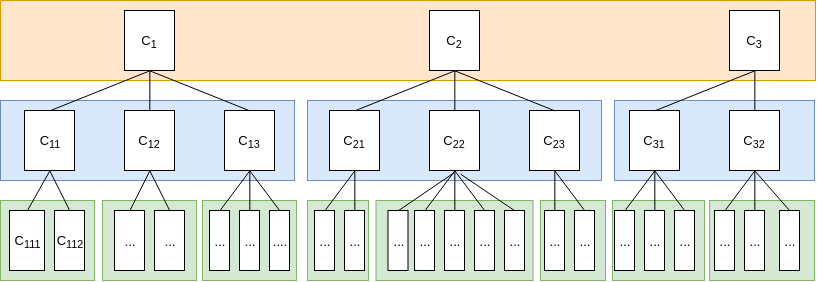
\includegraphics[width=\textwidth]{images/hierarchical_classification.png}
	

\end{frame}


\begin{frame}[label=metho]{Methodology}
	\textbf{Specializing Every Node}
	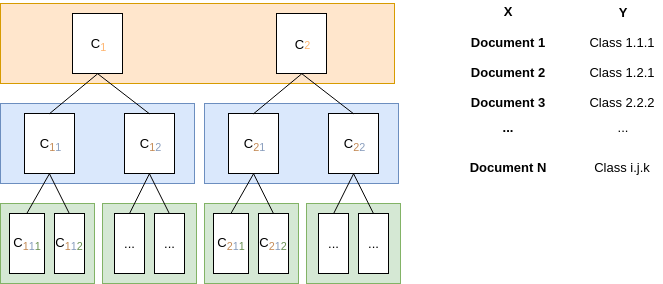
\includegraphics[width=\textwidth]{images/distribution_0.png}
\end{frame}


\begin{frame}[label=metho]{Methodology}
	\textbf{Specializing Every Node}
	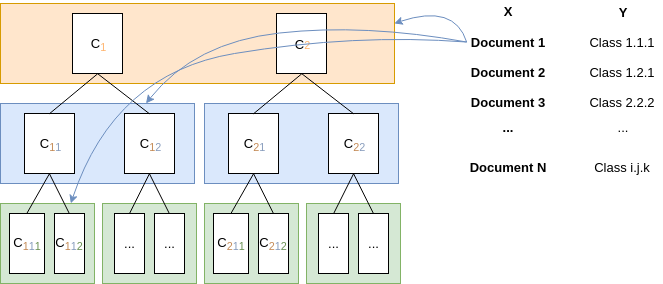
\includegraphics[width=\textwidth]{images/distribution_1.png}
\end{frame}

\begin{frame}[label=metho]{Methodology}
	\textbf{Specializing Every Node}
	
	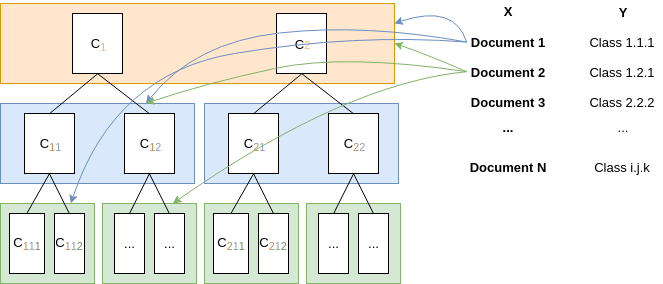
\includegraphics[width=\textwidth]{images/distribution_2.png}
	
	
\end{frame}


\begin{frame}[label=metho]{Methodology}
	\textbf{Specializing Every Node}
	
	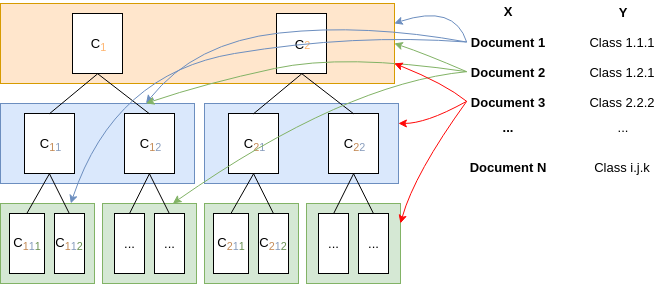
\includegraphics[width=\textwidth]{images/distribution_3.png}
	
\end{frame}


\begin{frame}[label=metho]{Methodology}
	\textbf{Wrap Up}
	
	\begin{itemize}
		\item Build a data set by extracting live data
		\item Train a multi layer hierarchical classifier
	\end{itemize}
	
\end{frame}


